\begin{table}[t]\centering\small
\begin{tabular}{@{\;}r@{ $\to$ }lll@{}} \toprule
\multicolumn{2}{c}{\textbf{Rule}} & \textbf{Semantics}
& \textbf{Example} \\ \midrule

$\C{TokenSpan}$ & $\C{Entity}$
& $\mathrm{fuzzymatch}(s)$
& $\T{China}$ \quad (from \nl{Chinese}) \\
\explainBLong{$\Mr{fuzzymatch(s)}$ generates cell nodes with string approximately matching $s$} \\

$\C{Values} + \C{ValueFn}$ & $\C{Values}$
& $S(z_1, z_2)$
& $\T{argmax}(\xOf{Event}.\T{allRows}, \lambda v[\T{count}(\xHas{Event}.v)])$ \\
\explainBLong{A \C{ValueFn}, as defined in Table~\ref{tab:sempre-compositional-rules},
maps cells or atomic values
into comparable values} \\

\bottomrule

\end{tabular}
\caption[Additional deduction rules to increase question coverage.]{
Additional deduction rules to increase the coverage
on answerable questions.
}\label{tab:macro-new-rules}
\end{table}

\begin{table}[t]
\centering
\begin{tabular}{ll} \toprule
\nl{Which driver appears the most?}
& $\T{argmax}(\xOf{Driver}.\T{allRows},
\lambda v[\T{count}(\xHas{Driver}.v)])$ \\
\nl{Is English for French spoken more?}
& $\T{argmax}(\T{English} \sqcup \T{French},
\lambda v[\T{count}(\xHas{Language}.v)])$ \\
\nl{Who is taller, Rose or Time?}
& $\T{argmax}(\T{Rose} \sqcup \T{Tim},
\lambda v[\xOf{Num}.\xOf{Height}.\xHas{Name}.v])$ \\
\bottomrule
\end{tabular}
\caption{Examples of superlative logical forms applied on sets of cell nodes.}
\label{tab:macro-superlative}
\end{table}

As mentioned at the end of the previous chapter (Section~\ref{sec:sempre-true-oracle}),
we would like to increase the coverage over
answerable questions by expanding the space
of logical forms that can be generated.
One way to achieve this is by expanding the
set of deduction rules.
In particular, we add new rules listed in
Table~\ref{tab:macro-new-rules},
which allows cells nodes to be generated
from approximate string matching
(e.g., the phrase \nl{Chinese} can now map to \T{China}),
and introduces superlatives on sets of cell nodes
as demonstrated in Table~\ref{tab:macro-superlative}.

Adding just these two rules
already increases the true oracle number
from 53.5\% %to \qqq\%.
by almost 10\% absolute.
This is because both rules directly address
the major coverage errors as analyzed in
Section~\ref{sec:sempre-error-analysis}.
However, since the added rules can potentially generate
many more candidate logical forms
(e.g., there can be multiple cells approximately
matching each utterance token span),
the increased coverage comes with a cost of
slower running time.
On average per example,
the training time increases from 619 ms to 1,117 ms,
and the prediction time increases from 645 ms to 1,150 ms.
This doubling of running time could mean additional days
to train and tune a model.
Even worse, the running time will increase even more
when the space of logical form is expanded further
to gain more question coverage.

%\section{Using patterns to guide search}

\begin{figure}[t]
\centering
\textsf{
\begin{tabular}{|c|c|c|c|c|} \hline
\textbf{Year} & \textbf{Venue} & \textbf{Position} & \textbf{Event} & \textbf{Time} \\ \hline
2001 & Hungary & 2nd & 400m & 47.12 \\
2003 & Finland & 1st & 400m & 46.69 \\
2005 & Germany & 11th & 400m & 46.62 \\
2007 & Thailand & 1st & relay & 182.05 \\
2008 & China & 7th & relay & 180.32 \\ \hline
\end{tabular}
}
\\[0.5em]
\begin{tabular}{r@{ }l}
$x=$ & \nl{Which location comes after Germany?} \\
$z=$ & $\xOf{Venue}.\xOf{Next}.\xHas{Venue}.\T{Germany}$ \\
$y=$ & \{\T{Thailand}\}
\end{tabular}
\caption{Our running example from before but with a different question.}
\label{fig:running-ex-macro}
\end{figure}

% As emphasized earlier,
% the need to handle open-domain web tables (\Breadth)
% and more complex questions (\Depth)
% causes the space of logical forms to explode quickly.
% In the previous chapter, we introduced methods
% to sidestep the issue
% by treating search as a preprocessing step.
% This chapter explores a different solution:
% following the original training method
% in Chapter~\ref{chp:parsing},
% we perform search during training,
% but we search more cleverly
% by using patterns of logical forms found in
% previously processed example to guide the search process.
% Our approach is based on two key ideas:

In this chapter,
we propose to speed up the parser
by making the search algorithm prioritize
logical forms that ``look good''
according to its past experience.
Our approach is based on two key ideas:

\begin{itemize}
\item
\textbf{Good logical forms share common patterns.}
%To give an intuition,
For example,
consider the question
\nl{Which location comes after Germany?}
for the table in Figure~\ref{fig:running-ex-macro}.
One possible semantically correct logical form is
\begin{equation}
\xOf{Venue}.\xOf{Next}.\xHas{Venue}.\T{Germany},
\end{equation}
%which executes to the correct answer \T{Thailand}.
which identifies the cell below \emph{Germany}
in the same \emph{Venue} column.
From this logical form,
we can abstract out question-specific and
table-specific predicates
(i.e., columns, cells, and primitive values) to get
the following \emph{macro}:
\begin{equation}
\aOf{\C{Col}\#1}.\xOf{Next}.\aHas{\C{Col}\#1}.\A{\C{Cell}\#2},
\end{equation}
which identifies the cell below $\A{\C{Cell}\#2}$
in the same $\A{\C{Col}\#1}$ column.
Such a macro captures a domain-independent
computational pattern
that generalizes across different table contexts.
The main idea of
our training procedure
is to extract macros
from logical forms found from search,
and then use them to efficiently construct
logical forms in new contexts.

\item
\textbf{Similar utterances are likely to share a
logical form pattern.}
Though the space defined by macros is smaller
than the original search space,
the set of extracted macros will eventually grow
with the number of processed examples.
To prioritize macros that are more likely to match
for the input question $x$,
we propose \emph{holistic triggering}:
find the $K$ examples with questions most similar to $x$,
and then only test macros extracted from
the consistent logical forms found in those examples.
\end{itemize}

Based on the two ideas above,
we propose an online learning algorithm
that jointly learns a semantic parser
and a set of macros
encoded as \emph{macro deduction rules}.
For each training example,
the algorithm first tries to find consistent logical forms
by using holistic triggering to invoke a subset
of promising macro rules to apply.
If it succeeds, the logical forms
are used to update the parameters of the semantic parser.
Otherwise, it falls back to the
base deduction rules to perform a more exhaustive search,
and then uses the discovered consistent logical forms
to derive more macro deduction rules.
At test time, we only use the learned macro deduction rules.

The next two sections describe the details of
macro deduction rules and the training algorithm.
Afterward, we evaluate our approach on the \wtq dataset
in terms of accuracy and speed.
Training with macro rules yields a 11x speedup
compared to training with the base deduction rules,
and at test time,
we achieve a slightly better accuracy of 43.7\%
with a 16x speedup compared to the baseline.

\paragraph{Reference.}
The results described in this chapter have been published as
\citet{zhang2017macro}.
Reproducible experiments are hosted on the
CodaLab platform at
\begin{center}
\small
\url{https://worksheets.codalab.org/worksheets/0x4d6dbfc5ec7f44a6a4da4ca2a9334d6e}.
\end{center}

\section{Macros}

\subsection{Deriving macros from logical forms}

\begin{figure}
\centering
\begin{subfigure}[b]{\textwidth}\centering
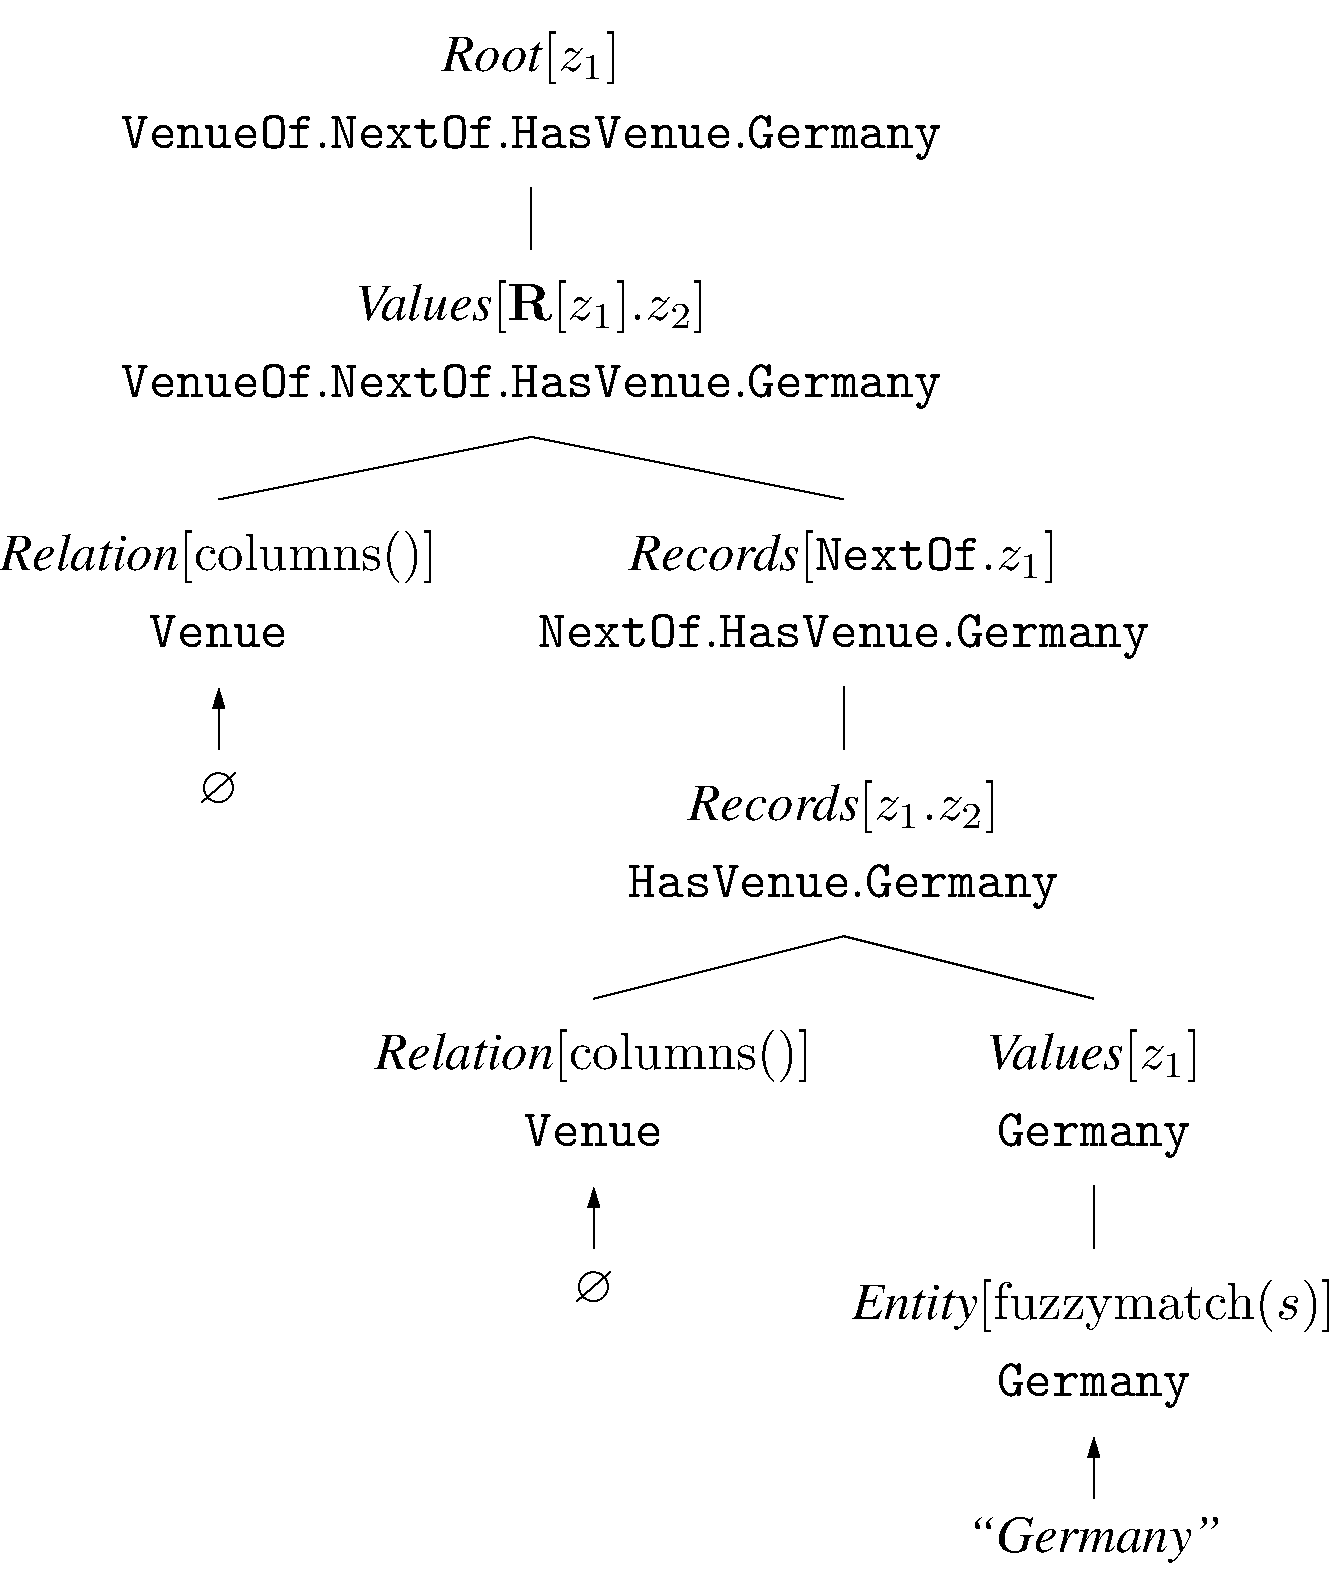
\includegraphics[scale=.35]{sfig/parsetrees.slides/macroParseOrig.pdf}
\caption{Derivation tree ($z_i$ represents the $i$th child)}
\label{fig:compute-macro-a}
\end{subfigure} \\[1em]
\begin{subfigure}[b]{0.40\textwidth}\centering
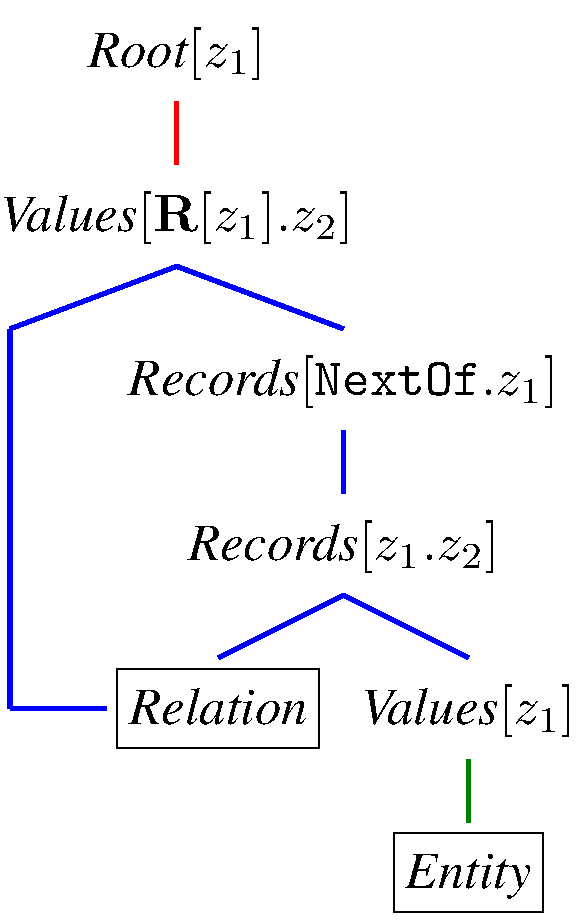
\includegraphics[scale=.35]{sfig/parsetrees.slides/macroParseMacro.pdf}
\caption{Macro}
\label{fig:compute-macro-b}
\end{subfigure}
\begin{subfigure}[b]{0.40\textwidth}\centering
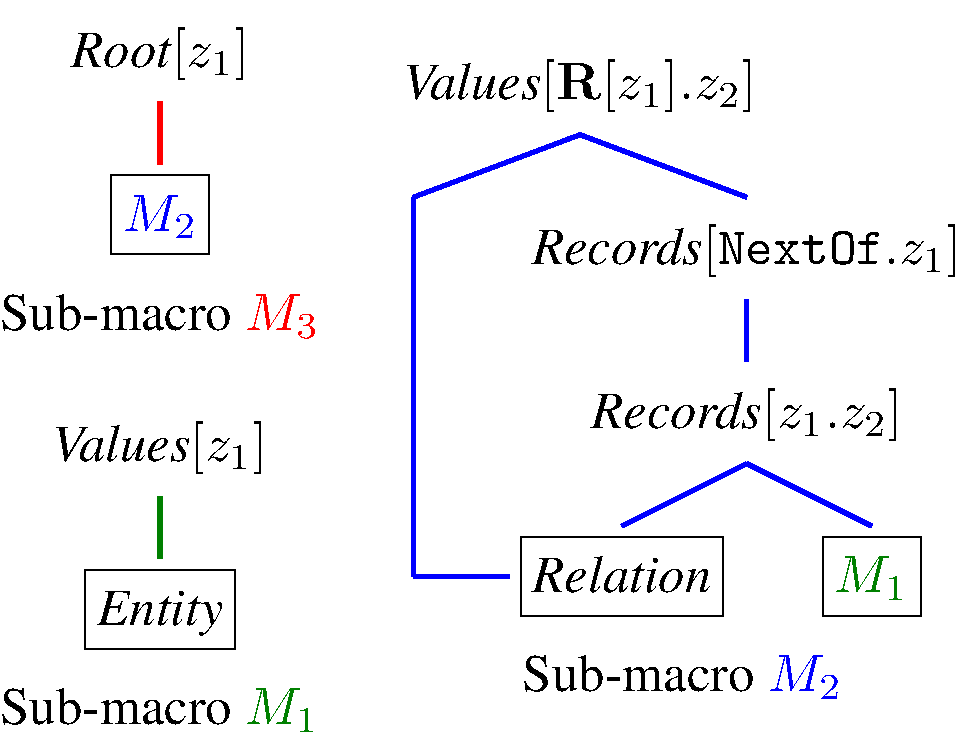
\includegraphics[scale=.35]{sfig/parsetrees.slides/macroParseSubMacros.pdf}
\caption{Atomic sub-macros}
\label{fig:compute-macro-c}
\end{subfigure}
\caption[
Derivation of macro deduction rules.
]{From the derivation tree (a), we extract a
macro (b), which can be further decomposed into
atomic sub-macros (c). Each sub-macro is converted
into a macro rule.}
\label{fig:compute-macro}
\end{figure}

A \emph{macro} $M$
characterizes an abstract logical form structure.
For any given logical form $z$,
we can compute its macro by transforming its derivation tree
as illustrated in Figure~\ref{fig:compute-macro}:
\begin{enumerate}
\item
For each terminal deduction rule (i.e., leaf node),
substitute it with a placeholder,
and label it with the category of that derivation
(i.e., the category on the right hand side of the
deduction rule).
\item
Merge leaf nodes that represent the same
partial logical forms.
For instance, the two mentions of \T{Nation}
in Figure~\ref{fig:compute-macro-b}
are merged to signify that the two column names
have to be identical.
\end{enumerate}

The resulting macro $M$ can be serialized as a flat string
by assigning an index to each placeholder
as illustrated in the figure.
While the resulting macro is not a tree,
we will use the terms \emph{root} and \emph{leaf}
to refer to nodes that were roots or leaves
in the original derivation tree.

A logical form $z'$ satisfies the macro
if it can be obtained by filling each placeholder in $M$
with a value of the matching category.
For instance,
the logical form
$z' = \xOf{Year}.\xOf{Next}.\xHas{Year}.\T{1st}$
satisfies the macro $M$ in the figure
(even though it executes to an empty set).

\subsection{Macro deduction rules}
For any macro $M$, we can construct a set of
\emph{macro deduction rules} that,
when combined with terminal rule from the 
original set of deduction rules
(called ``base deduction rules'' henceforth),
generates exactly the logical forms that satisfy
the macro $M$.
The most basic approach is to construct a single rule
for the whole macro:
if the placeholders of $M$ are labeled $c_1, \dots, c_k$,
we construct a deduction rule
\begin{equation}
c_1[z_1] + \dots + c_k[z_k] \to
\C{Root}[f(z_1, \dots, z_k)]
\end{equation}
where $f(z_1, \dots, z_k)$
is a semantic function that substitute $z_1, \dots, z_k$
to the corresponding placeholder nodes of $M$.
For example, the macro in Figure~\ref{fig:compute-macro-b}
yields a deduction rule
\begin{equation}
\C{Relation}[z_1] + \C{Entity}[z_2] \to
\C{Root}[\Mb{R}[z_1].\xOf{Next}.z_1.z_2]
\end{equation}

\paragraph{Decomposed macro deduction rules.}
To speed up the model,
we want to avoid processing the same
logical form fragment more than once.
For instance,
when we use macro deduction rules to generate
\begin{equation}
\T{max}(\xOf{Num}.\xOf{Year}.\xHas{Position}.\xHas{Num}.\C{1})
\end{equation}
and
\begin{equation}
\xOf{Venue}.\T{argmin}(\xHas{Position}.\xHas{Num}.\C{1},
\lambda r.\xOf{Index}.r),
\end{equation}
we want to avoid constructing and featurizing
the same fragment $\xHas{Position}.\xHas{Num}.\C{1}$
multiple times.
%
To achieve this goal,
we decompose macros $M$ into \emph{sub-macros}
and define deduction rules from them.
A subgraph $M'$ of $M$ is a sub-macro of $M$ if
\begin{enumerate}
\item $M'$ contains at least one non-leaf node
\item $M'$ connects to the rest of the graph ($M\setminus M'$)
only through the root of $M'$.
\end{enumerate}
A macro $M$ is \emph{atomic} if its only sub-macro is itself.
The process of decomposing a non-atomic macro $M$,
as illustrated in Figure~\ref{fig:compute-macro-c},
is as follows:
\begin{enumerate}
\item 
Detach an atomic sub-macro $M'$ from $M$
and define a macro rule
\begin{equation}
c'_1[z_1] + \dots + c'_k[z_k] \to c'_\Mr{out}[f(z_1, \dots, z_k)]
\end{equation}
where $c'_1, \dots, c'_k$
are the categories of the leaf nodes of $M'$,
and $f(z_1, \dots, z_k)$ is a semantic function
that substitutes $z_1, \dots, z_k$ into the macro $M'$.
The name of the category $c'_\Mr{out}$
is computed by serializing $M'$ as a string;
this way, if the sub-macro $M'$
appears in a different macro,
the category name will be shared,
and any logical form satisfying $M'$ will only be
constructed once.
\item
Substitute the subgraph $M'$ in $M$
by a placeholder node with name $c'_\Mr{out}$.
\item
Repeat Steps 1 and 2 on the new graph
until we are left with an atomic macro,
and define a final macro deduction rule for it.
\end{enumerate}

\section{Training algorithm}

\begin{algorithm}[t]\setstretch{1.1}
\caption{Process a training example with macro rules}
\label{alg:macro-algorithm}
\begin{algorithmic}[1]
\Require training example $(x, w, y)$, macro rules,
base rules with terminal rules $\Mc{T}$
\State Select a set $\Mc{R}$ of macro rules based on $x$ with holistic triggering
\State Generate a set $\zx$ of candidate logical forms
from rules $\Mc{R} \cup \Mc{T}$
\If {$\zx$ contains consistent logical forms}
\State Update model parameters
\Else
\State Apply the base rules to search for a consistent
logical forms
\State Augment the macro rules
\EndIf
\State Associate utterance $x$ with the highest-scoring
consistent logical form found
\end{algorithmic}
\end{algorithm}

We now describe an online algorithm
that jointly learns the semantic parser
and macro deduction rules.
Algorithm~\ref{alg:macro-algorithm}
describes how our algorithm proceeds
for each training example $(x, w, y)$.
It first tries to use a subset of macro deduction rules
to search for logical forms.
If the search succeeds,
then the semantic parser parameters are updated as usual.
Otherwise, it falls back to the base deduction rules,
and then add new macro rules based on the
consistent logical forms found.

\subsection{Holistic triggering}
\label{sec:macro-trigger}

The first step of our algorithm is to
select a subset $\Mc{R}$ of macro rules
that are likely to generate consistent logical forms
for the question $x$.
The selection is done as follows.
Throughout training,
we maintain a mapping $\Mc{S}$
from each previously processed question
to a consistent logical form found while processing that question.
(Questions for which
a consistent logical form has not been found
are not included.)
Given a new training question $x$,
we identify $K$ questions in $\Mc{S}$
that are the most ``similar'' to $x$
(i.e., $K$-nearest neighbors of $x$ under some similarity metric),
and then let $\Mc{R}$
be the set of macro deduction rules that
were extracted from their associated logical forms.

\paragraph{Question similarity metric.}
We use token-level Levenshtein distance as
the distance metric for computing the nearest neighbors.
To compute the distance between two sentences $x$ and $x'$,
we first preprocess them by lemmatizing the tokens,
and then removing all determiners and infrequent nouns
that appear in less than 2\% of the training questions.
The distance is then defined as the Levenshtein distance
between the two sequences of remaining tokens.
For instance, \nl{\textbf{Who} ranked \textbf{right after} Germany}
and \nl{\textbf{Who} took office \textbf{right after} Uriah Forrest}
have distance 4.
Despite its simplicity, our distance is good at
capturing structural similarity between questions.

To speed up training,
we pre-compute a sorted list of $K_\Mr{max} = 100$
nearest neighbors for every question in the training data.
When processing a question $x$ during training,
we calculate $\Mc{R}$ as
the intersection of the pre-computed list for $x$
and the set of questions in $\Mc{S}$.

\subsection{Updating the macro rules}
The computed subset $\Mc{R}$ of macro deduction rules
is combined with the set $\Mc{T}$ of base terminal rules
(for building basic units such as \C{Cell} and \C{Col}).
The floating parser parses the training question $x$
using deduction rules $\Mc{R} \cup \Mc{T}$,
resulting in a set $\zx$ of logical forms
(Line~2 of Algorithm~\ref{alg:macro-algorithm}).

If $\zx$ contains a consistent logical form,
we update the model parameters as usual
(Line~4);
otherwise, we fall back to performing
beam search using the base rules
(Line~6).
For efficiency, we stop the search
either when a consistent logical form is found,
or when the total number of generated logical forms
exceeds some threshold $T$.
These early stopping criteria prevent
the model from spending too much time on
difficult examples
(e.g., when the context table is large).
While we might miss consistent logical forms
and thus their macros on such examples,
we could potentially induce the same macro
from more straightforward examples.

When the algorithm succeeds at finding a consistent
logical form $z$ with the base rules,
we extract its macro $M$
and construct the corresponding decomposed macro rules
(Line~7).
Parameters of the parser are not updated
when the beam search with base rules is invoked.

Finally, if a consistent logical form $z$ is found,
the mapping $\Mc{S}$ is updated to map $x$ to $z$
(Line~8).

\subsection{Prediction}
At test time,
we follow steps 1--2
of Algorithm~\ref{alg:macro-algorithm}
to generate a set $\zx$ of candidate logical forms
from the triggered macro rules
and base terminal rules.
We then output the highest-scoring logical form $z \in \zx$.
We do not fall back to beam search at test time.

\section{Experiments}

We evaluate our approach on the \wtq dataset.
In addition to the test accuracy,
we will also compare the running times
during both training and test time.

\paragraph{Model details.}
We use the same features and logical form pruning strategies
from Chapter~\ref{chp:parsing}.
We use a beam size of $B = 100$ for beam search,
and use $K = 40$ for the $K$-nearest neighbor
in holistic triggering.
We take 3 passes over the training data during training.
When falling back to beam search,
we stop the search when the number of generated logical forms
reaches $T = 5000$ in the first pass.
To further increase speed,
we disallow falling back to beam search
during the subsequent passes
(which means that no more macro deduction rules
are constructed after the first pass).

\subsection{Main results}

\begin{table}[t]\centering
\begin{tabular}{lcc}\toprule
& \textbf{Dev} & \textbf{Test} \\ \midrule
Original deduction rules (Chapter~\ref{chp:parsing}) & 37.0\%	&37.1\%\\
% \citet{neelakantan2016neural}	&37.5\%&	37.7\%\\
% \citet{haug2017neural}	&-&	38.7\%\\\hline
New deduction rules	& \textbf{40.6\%}	&42.7\%\\
New deduction rules + macros & 40.4\%	& \textbf{43.7\%} \\
\bottomrule
\end{tabular}
\caption{Results of learning with macros on the \wtq dataset.
}\label{tab:macro-accuracy}
\end{table}

\newcommand{\midhead}[1]{\multicolumn{1}{c}{\textbf{#1}}}
\begin{table}[t]
\centering
\begin{tabular}{lrrr}
\toprule
& & \multicolumn{2}{c}{\textbf{Time (ms/ex)}} \\ \cmidrule{3-4}
& \midhead{Acc.} & \midhead{Train} & \midhead{Pred} \\
\midrule
Original deduction rules (Chapter~\ref{chp:parsing})
& 37.0\% & 619 & 645 \\
New deduction rules & \textbf{40.6\%} & 1,117 & 1,150 \\
New deduction rules + macros & 40.4\%  & \textbf{99} & \textbf{70} \\
\quad no holistic triggering & 40.1\% &  361 & 369 \\
\quad no macro decomposition & 40.3\% & 177 & 159 \\
\bottomrule
\end{tabular}
\caption[Running time of macro rules]
{Comparison and ablation study. The columns report averaged prediction accuracy, training time, and prediction time (milliseconds per example) on the three development splits.}\label{tab:macro-time}
\end{table}

\paragraph{Test accuracy.}
Table~\ref{tab:macro-accuracy} shows the test accuracy
of our approach and other parses on the \wtq dataset.
Compared to the original floating parser,
learning with macros slightly improves the test accuracy
from 42.7\% to 43.7\%,
while the averaged development accuracy on three development splits
are similar for the two approaches
(40.6\% vs 40.4\%).

\paragraph{Running time.}
Table~\ref{tab:macro-time} lists the
running time needed to process an example
in the original floating parser
and our new approach.
We trained all parsers on a machine
with Xeon 2.6GHz CPU and 128GB memory without parallelization.
Learning with macros is substantially
more efficient, with 11x speedup during training
and 16x speedup at test time.

\paragraph{Ablation analysis.}
We run two ablations of our algorithm:
removing holistic triggering
(i.e., consider all macro rules when parsing a question $x$)
and removing macro decomposition
(i.e., construct a single deduction rule for each macro).
Table~\ref{tab:macro-time}
shows that the ablated models are slower
to process examples.
This is because holistic triggering
greatly narrows down
the set of macro rules for parsing questions,
while decomposed macro rules
save us from featurizing the same
logical form fragments multiple times.

\subsection{Coverage of macros}
Using the base deduction rules,
the floating parser generates an average of 13,700
partial logical forms for each training example,
and discovers a consistent logical form
in 81.0\% of the examples.
When learning with macros,
the numbers become 1,300 and 75.6\%.

At a first glance,
learning with macros seems to
reduce the coverage of logical forms,
but this is untrue once we factor out spurious logical forms
(i.e., logical forms that execute to the right denotation
for wrong reasons).
% However, the discovered consistent logical forms
% also include spurious logical forms.
To measure the coverage over semantically correct logical forms,
we turn to the 300 examples that
we annotated with correct logical forms in Chapter~\ref{chp:dpd}.
We find that for 48.7\% of these examples,
the top consistent logical form produced
by the base deduction rules is semantically correct
(i.e., exactly matches
or is equivalent to the annotated logical form).
When learning with macros,
the number stays at 48.7\%,
meaning that the effective coverage
of the learned macro deduction rules
is as good as the base ones.


% \begin{table}\centering
% \input{figures/wtq/top-macros.tex}
% \caption{Top macros learned from the \wtq dataset and their semantics.}
% \label{tab:macros-top-macros}
% \end{table}

% \paragraph{Extracted macros.}
% Our approach extracts 123 macros in total.
% Among the training examples
% that the algorithm can find a consistent logical form,
% the top 34 macros listed in Table~\ref{tab:macros-top-macros} cover 90\%
% of those logical forms.

\subsection{Influence of hyperparameters}

\begin{figure}[t]
\begin{subfigure}[b]{0.333\textwidth}\centering
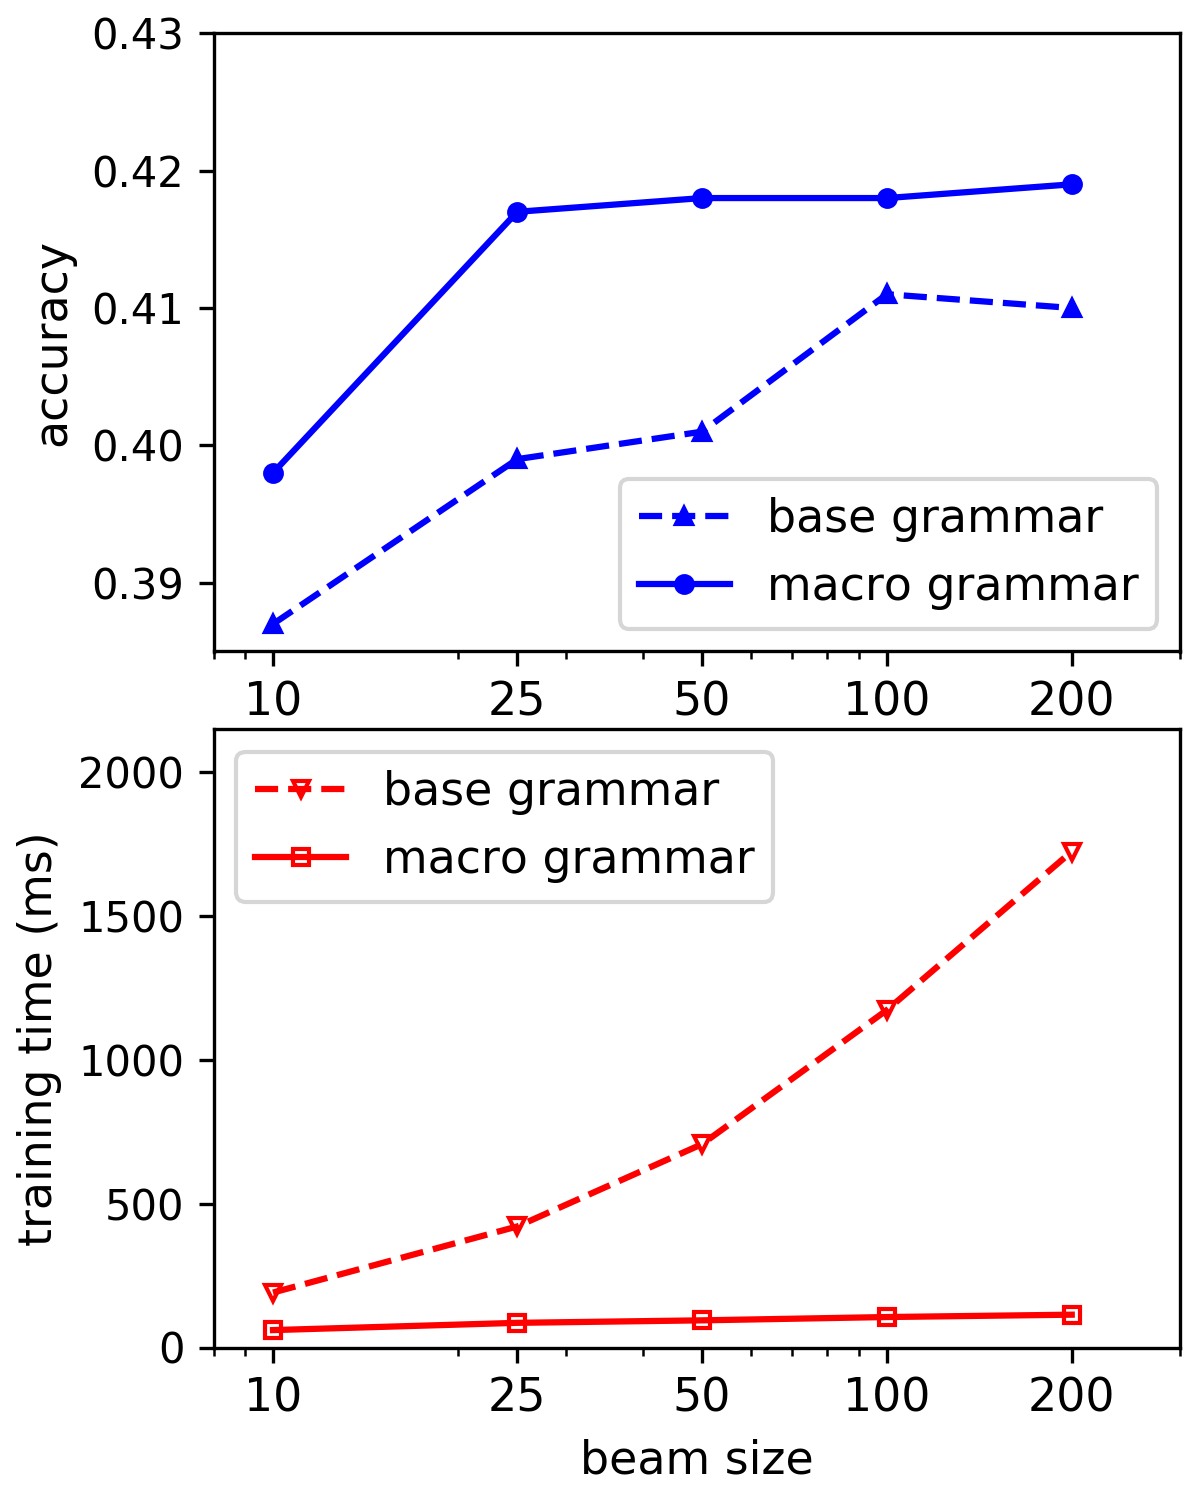
\includegraphics[width=1.0\linewidth]{figures/wtq/beamsize_split_high.png}
\caption{Varying beam size}
\label{fig:macro-hyperparam-a}
\end{subfigure}%
\begin{subfigure}[b]{0.333\textwidth}\centering
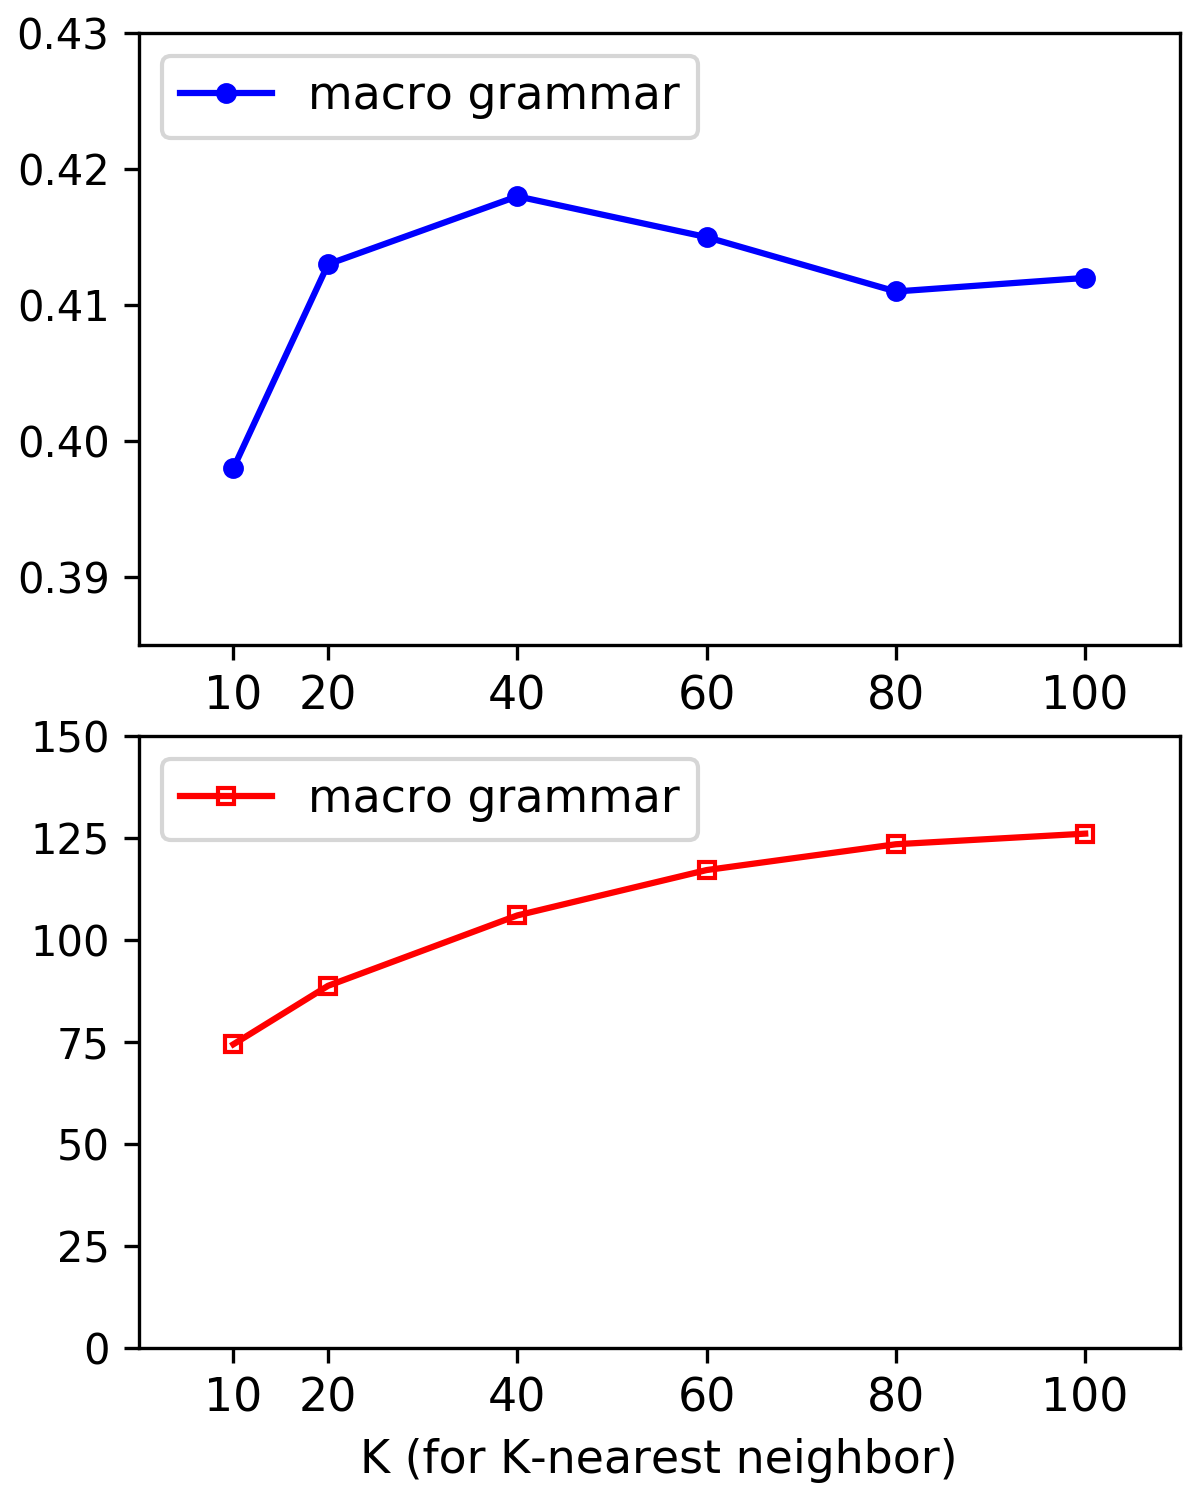
\includegraphics[width=1.0\linewidth]{figures/wtq/nn_k_split_high.png}
\caption{Varying neighbor size}
\label{fig:macro-hyperparam-b}
\end{subfigure}%
\begin{subfigure}[b]{0.333\textwidth}\centering
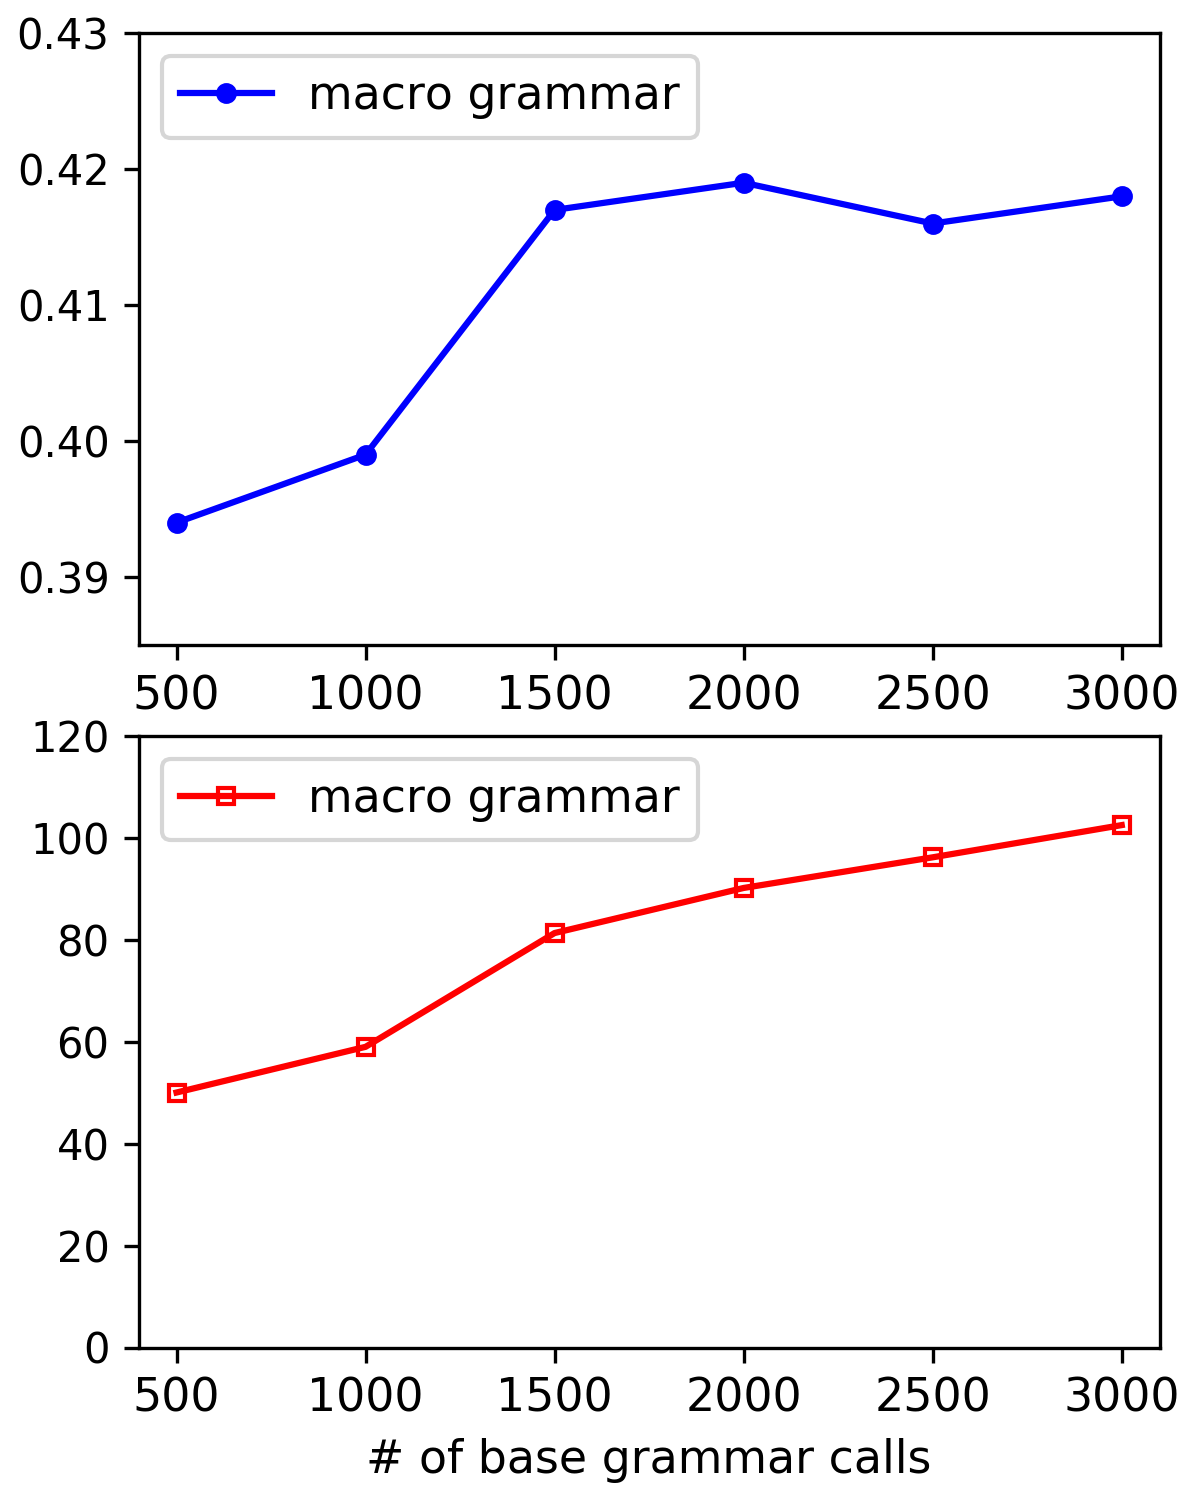
\includegraphics[width=1.0\linewidth]{figures/wtq/max_exploration_split_high.png}
\caption{Varying base rules usage count}
\label{fig:macro-hyperparam-c}
\end{subfigure}
\caption[Accuracy and training time with various hyperparameter choices]{
Accuracy and training time (per example) with various
hyperparameter choices, reported on the first train-dev split.
}\label{fig:macro-hyperparam}
\end{figure}

We compare the accuracy and training time per example
on the first development split of the dataset
when hyperparameters varies.

\paragraph{Beam size.}
Figure~\ref{fig:macro-hyperparam-a}
shows that for all beam sizes $B$,
training with macros is more efficient than
with the base deduction rules,
and the speedup rate grows with beam size.
The accuracy is robust to the varying beam size
as long as $B \geq 25$.

\paragraph{Number of neighbors in holistic triggering.}
We now consider $K$,
the number of neighboring questions
when computing the subset $\Mc{R}$ of macro rules
in Section~\ref{sec:macro-trigger}.
Figure~\ref{fig:macro-hyperparam-b}
shows that retrieving fewer similar questions
speeds up training but decreases accuracy.
On the other hand,
retrieving too many similar questions
can overload the list $\Mc{R}$
with potentially spurious macros,
which could explain why the accuracy
slightly drops when $K$ is too high.

\paragraph{Number of fallback searches.}
We perform ablation experiments
where we limit the number of times
that the algorithm can fall back to 
beam search on base deduction rules to at most $m$ times.
This effectively limits the number of macros
that the algorithm can discover:
the set of macro rules will be augmented 
at most $m$ times.
With smaller $m$, the accuracy grows with $m$,
which suggests that discovering a richer set of macros
improves the accuracy.

However, the accuracy changes much more slowly
once $m$ hits 1,500.
This suggests that we could speed up the model
even further by stopping the model from
finding macros after it has processed
some fraction of the training data.
Indeed, we try training a model with $B = 50$,
$K = 40$, and $m = 2000$.
The resulting model reduces the development accuracy
very slightly (down from 40.4\% to 40.2\%),
but it achieves more speed up during both training time
(up from 11x the base floating parser to 15x)
and test time
(up from 16x to 20x).

\section{Related work and discussion}

\paragraph{Modeling recurring structures.}
A few generative models have been proposed
to model recurring structures.
Examples of these models include adaptor grammars
\cite{johnson06adaptor}
and fragment grammars
\cite{odonnell11fragment},
which were designed to assign
higher probabilities to the structures
that use the reoccurring parts.
One example application of such models in semantic parsing
is the idiom-based program synthesis work by \citet{iyer2019learning},
where the common program idioms,
such as nested for-loops,
can be extracted from a large
library of unlabeled data.
The idioms are then added to the set of possible
production rules in a similar way to how
we add macro rules (without decomposition).
And like how our macro rules are used,
the idiom can be invoked during decoding
to produce a whole section for the desired program.

The main difference between our macro grammar
and these generative models
is that the generative models aim to improve modeling,
using the intuition that
learning to predict the repeating structure as a single action
is easier than learning to generate all parts.
% Since we only have distant supervision,
% our approach learns such idioms in an online fashion.
In contrast, our training algorithm
caches the patterns only to speed up search,
while the score assignment is done by a discriminative
scorer.
Nevertheless, we also notice a slight modeling improvement
on the test data.

\paragraph{Explicit mapping of phrases to logical form patterns.}
Previous semantic parsing work
has proposed a few methods to infer explicit
mappings from utterance phrases to logical form patterns.
For instance, the higher-order unification method
\cite{kwiatkowski10ccg,kwiatkowski11lex}
learns such a mapping in an online fashion
during training.
The result is a lexicon where each entry
contains a logical form template and a set of possible phrases
for triggering the template.

Our macros are triggered not by explicit mappings,
but instead use holistic triggering to
over-suggest the plausible macros to use.
This is similar to how the floating parser generates
some predicates independently from the utterance
with a soft guidance from the scorer.
This allows us to generate logical forms for utterances
containing unseen lexical paraphrases.
Moreover, our holistic triggering also works
when the triggers is not a local contiguous part
of the utterance.
For instance, the question
\nl{\textbf{Who is} older, Jack \textbf{or} John?}
can trigger the macro learned from
\nl{\textbf{Who is} taller, Rose \textbf{or} Tim?}:
the logical form pattern of applying \T{argmax}
on the union of two entities is dependent on the
whole structure of the sentence.

\paragraph{Sketch-based and retrieval-based program synthesis.}
The process of producing a logical form pattern
and filling in the details
is closely related to sketch-based program synthesis
\cite{solar05sketching}.
To generate a program,
the program sketch containing placeholders
is first chosen,
and then a synthesis algorithm
(search-based or solver-based)
is used to find the values for the placeholders
that make the program satisfy the program specification.
This technique has been
recently applied in the context of
neural semantic parsing
\cite{dong2018coarse},
where both the sketch and the actual logical forms
are generated using neural decoders:
the sketch is first generated based on the input,
then a second network encodes the sketch
and decodes the actual logical form.
When the target logical form is available,
the sketch can be directly inferred
and used to train the sketch generator.
In our case, we use the logical forms found by beam search
to create macros (cf.\ sketches),
and the macros in turn helps make search faster.

Another related approach is retrieval-based synthesis
\cite{gu2017search,hayati2018retrieval,guu2018edit}.
To generate an output for the current input $x$,
the output $y'$ of a similar input $x'$ in the corpus
is retrieved, and then the model uses $y'$
to generate an output $y$ for our input $x$.
Unlike our work which derives and caches macros,
these retrieval-based approaches can use the raw corpus
without having to preprocess it.

\section{Conclusion}
We have presented an algorithm to speed up both the
training and prediction time of our floating parser.
Under the assumption that logical forms
for similar utterances tend to share
the same pattern,
we use macro deduction rules to encode logical form patterns,
and use holistic triggering to choose the macro rules
that are the most relevant for the question.
Our approach can trade off between 
exploitation (applying macro deduction rules)
and exploration (falling back to beam search)
to achieve a large speed up without sacrificing the accuracy.
This allows us to efficiently expand the deduction rules
and knowledge graph representation so that more types of questions
can be answered.

One downside of our approach is that,
as a caching mechanism,
the macro rules do not kick in during the beginning of
the training process.
For the first few training examples,
not many macro rules have been accumulated,
which curtails the level of speed up seen in the final experiments.
Even worse, during early training iterations,
the parameters of the scoring function
are still not well-calibrated.
This leads to beam search pruning away
essential logical form parts,
and thus we are less likely to find a consistent logical form
when falling back to beam search.

% Since the distant supervision from annotated answers
% requires us to search over logical forms during training,
% we can get rid of search problems by
% changing the type of supervision.
% In the next chapter, we will explore techniques for converting
% the distant supervision (denotations) in the dataset
% to direct supervision (logical forms).
% While the conversion process also involves a search algorithm,
% additional information from the annotated answer
% and minimal crowdsourcing will allow us to
% overcome of the challenges when searching over the space
% of logical forms.
